%%%%%%%%%%%%%%%%%%%%%%%%%%%%%%%%%%%%%%%%%%%%%%%%%%%%%%%%%%%%%%%
%
% Welcome to Overleaf --- just edit your LaTeX on the left,
% and we'll compile it for you on the right. If you open the
% 'Share' menu, you can invite other users to edit at the same
% time. See www.overleaf.com/learn for more info. Enjoy!
%
%%%%%%%%%%%%%%%%%%%%%%%%%%%%%%%%%%%%%%%%%%%%%%%%%%%%%%%%%%%%%%%


% Inbuilt themes in beamer
\documentclass{beamer}
\newcommand{\mydet}[1]{\ensuremath{\begin{vmatrix}#1\end{vmatrix}}}
\usepackage[super]{nth}
\usepackage{amsmath}
% Theme choice:
\usetheme{CambridgeUS}

% Title page details: 
\title{Assignment 2}% \\ Indian Institute of Technology Hyderabad} 
\author{Malothu Avinash \\ AI21BTECH11018}
\date{\today}
% \logo{\large \LaTeX{}}


\begin{document}

% Title page frame
\begin{frame}
    \titlepage 
\end{frame}

% Remove logo from the next slides
% \logo{}


% Outline frame
\begin{frame}{Outline}
    \tableofcontents
\end{frame}


% Lists frame
\section{Question}
\begin{frame}{Question}
A person buys a lottery ticket in 50 lotteries ,in each of which his chance of winning a prize is 1/100.What is the probability that he will win a prize
(a)at least once
    
(b)exactly once
    
(c)at least twice
\end{frame}

\section{Answer}
\begin{frame}{Answer}
(a)Let X represents the number of prizes winning in 50 lotteries and the trials are Bernoulli trails.

Here,We have a binomial distribution where n=50 p=1/100 then
\begin{align}
  &q=1-p\\
  &q=1-1/100\\
  &q=99/100
\end{align}
  As\;we\;know\;
  &P(X=x)={}^{n}C_{x}\cdot q^{n-x} \cdot p^x


\end{frame}
\begin{frame}
\begin{align}
    &={}^{50}C_{x}\cdot (\frac{99}{100})^{n-x} \cdot (\frac{1}{100})^x
   \\&\text{Hence the probability of winning lottery at least once is}\\
   &=P(X\geq1)\\
   &=1-P(X<1)\\
   &=1-P(X=0)\\
   &=1-{}^{50}C_{0}\cdot (\frac{99}{100})^{50}\\
   &\text{We get final probability as}=1-(\frac{99}{100})^{50}\\
\end{align}
\end{frame}
\begin{frame}
\begin{align}
   &\text{(b) The probability of winning lottery exactly once is }\\
   &=P(X=1)\\
   &={}^{50}C_{1}\cdot (\frac{99}{100})^{49}\cdot(\frac{1}{100})^1\\
   &\text{We get final probability as}=\frac{1}{2}\cdot(\frac{99}{100})^{49}\\
\end{align}
\end{frame}
\begin{frame}
\begin{align}
       \\&\text{(c)The probability of winning lottery at least twice is}\\
   &=P(X<2)\\
   &=1-P(X\leq1)\\
   &=1-[P(X=0)+P(X=1)]\\
   &=[1-P(X=0)]-P(X=1)\\
   &=1-(\frac{99}{100})^{50}-\frac{1}{2}\cdot(\frac{99}{100})^{49}\\
   &=1-(\frac{99}{100})^{49}\cdot[\frac{99}{100}+\frac{1}{2}]\\
   &\text{We get final probability as}=1-(\frac{149}{100})\cdot(\frac{99}{100})^{49}
\end{align}

\end{frame}
\begin{frame}{Code Output:}
The following is a result of python code plotting pmf of given cases
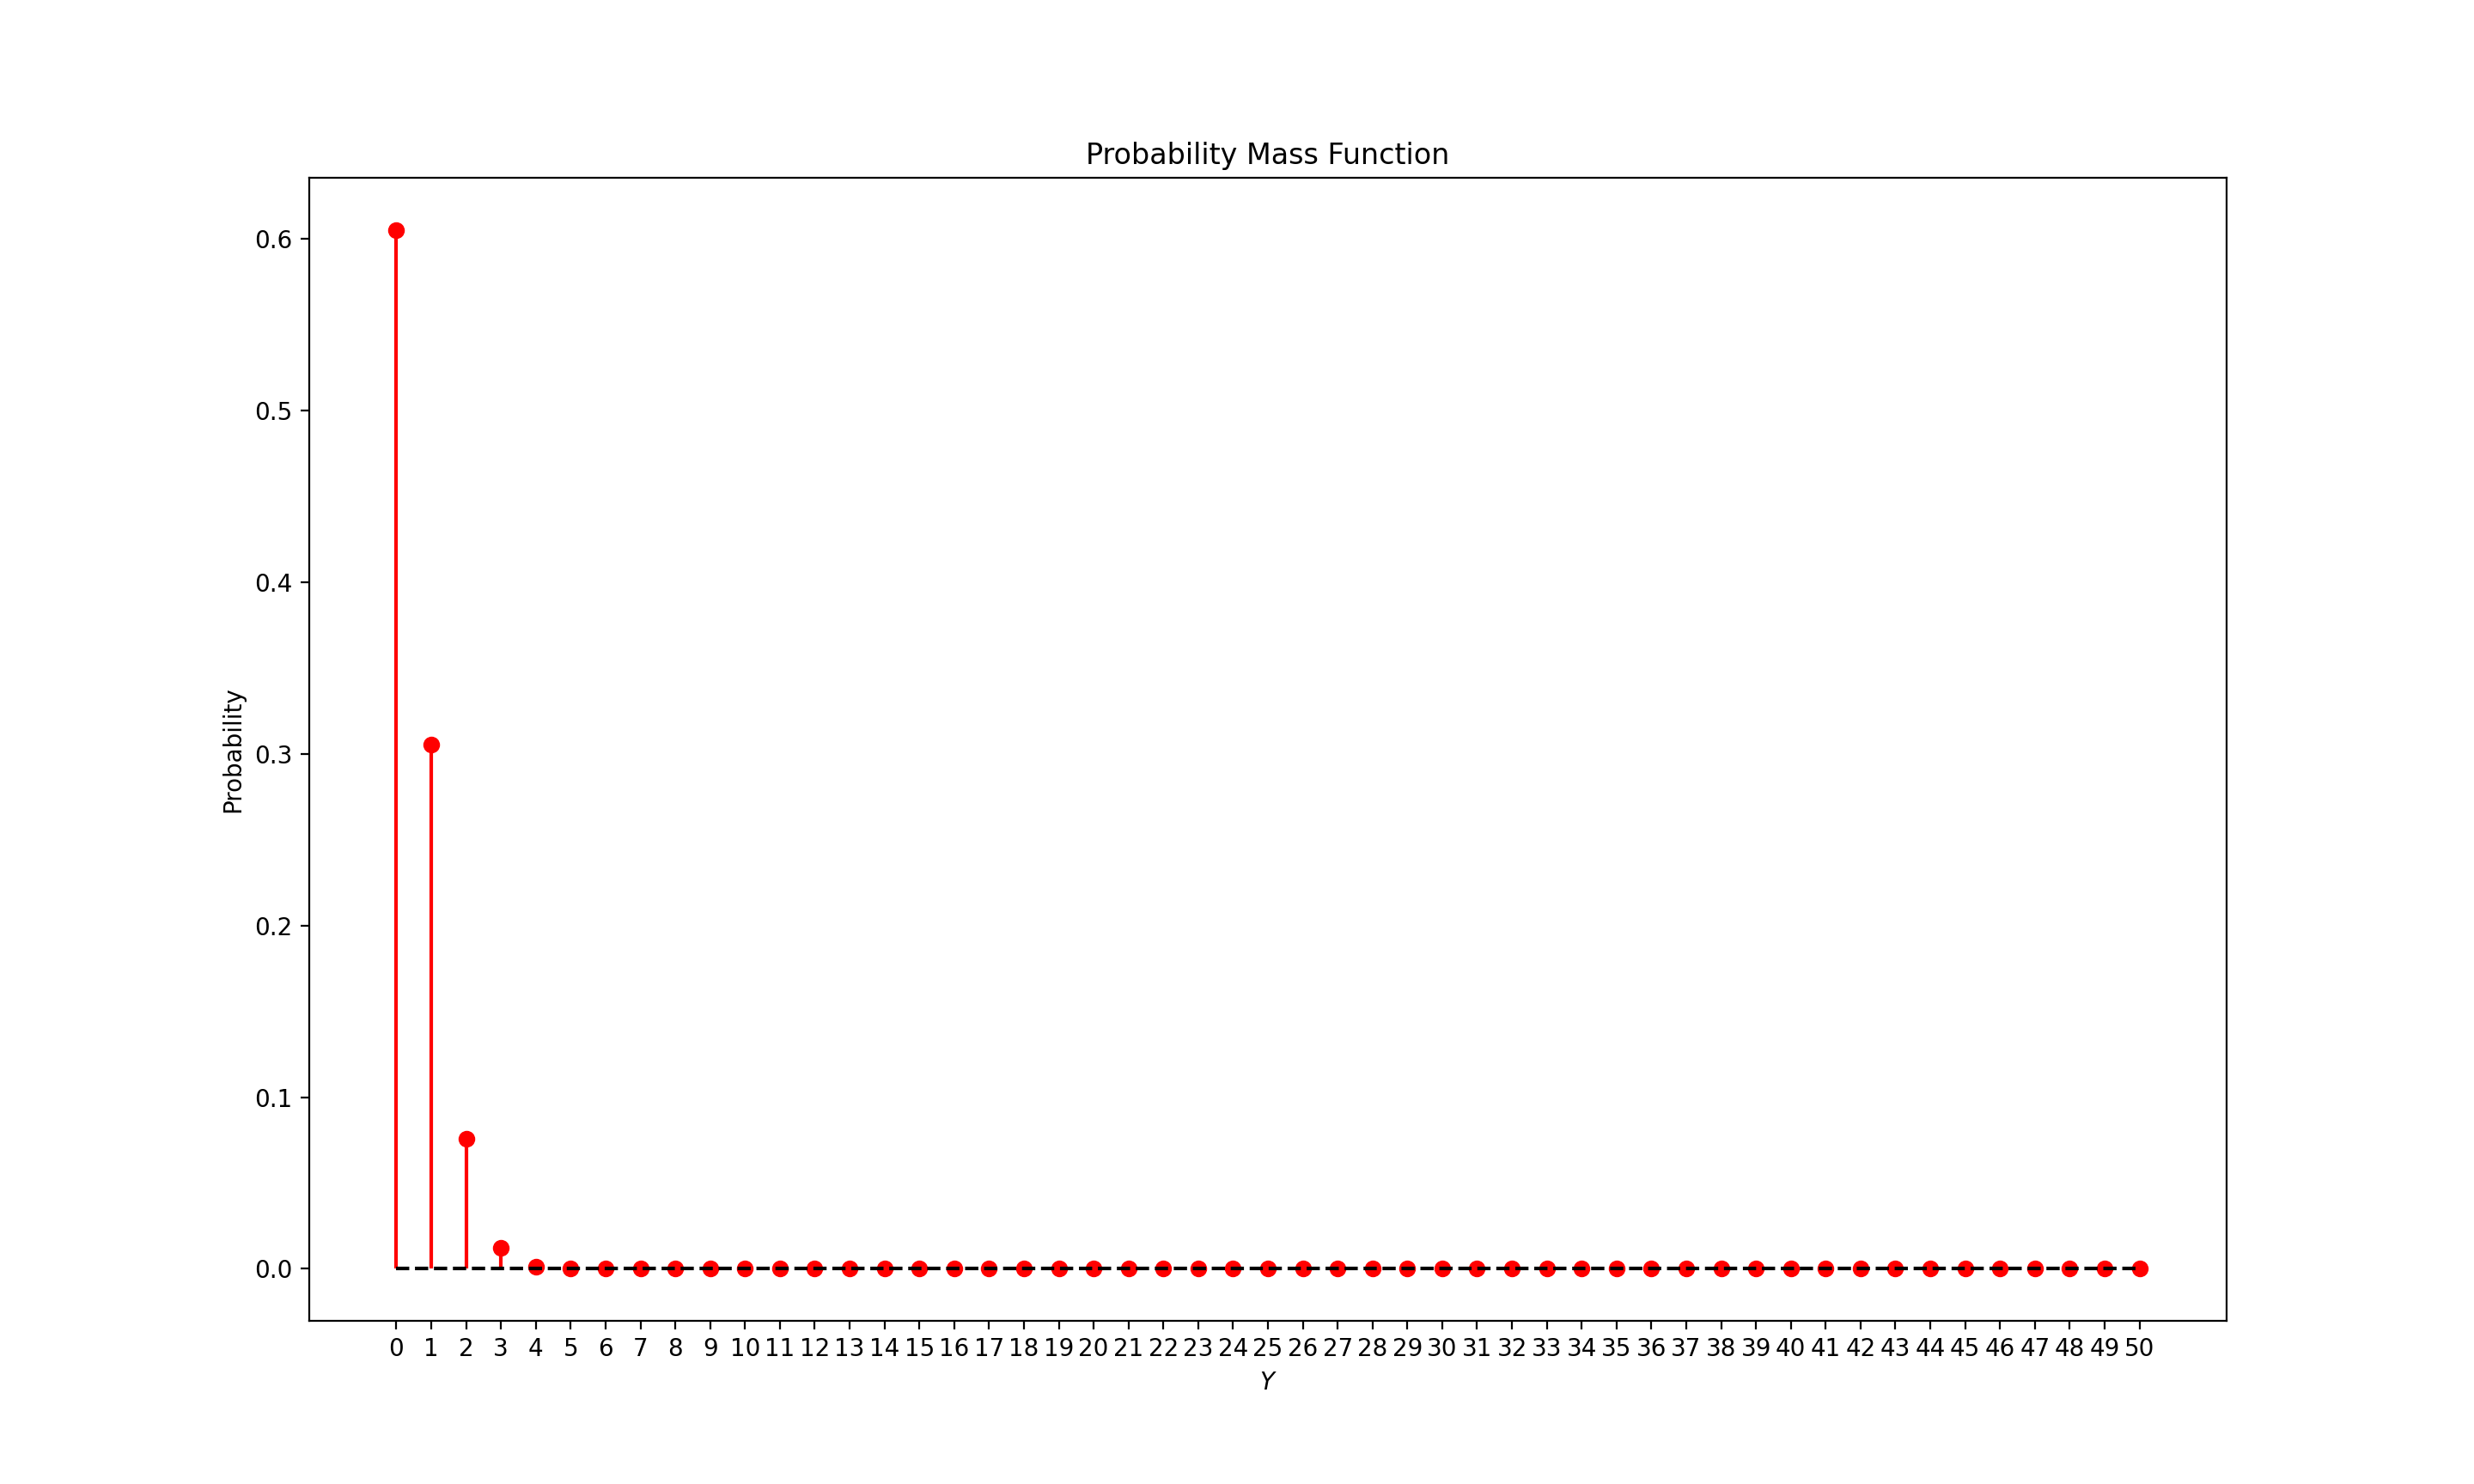
\includegraphics[width=\paperwidth]{Figure_1.png}
\end{frame}

\end{document}
